\chapter{Implementation}
\label{chap:implementation}
This Chapter is focused around the challenges the group met during development and how these were solved.  

\section{Limited field of view}
As mentioned in Section~\ref{sec:fieldOfView} the game contains a component that creates a view mesh, and uses a shader on this mesh that utilizes the stencil buffer for a per pixel masking. Any other object in our game that should be masked out in the fog of war also needs a different shader that implements the stencil buffer for masking. Having the fog of war was a design decision to limit the player's field of view, and give them imperfect information, which emulates how it would be in any first person game.\cite{gameDesignTheory}
Since the stencil buffer is a binary masking, the area outside of the view mesh would be completely dark. Even if this also enforces the fps view, it makes traversal around the map difficult.

\todo{Our additions to the code}

\section{Responsive user experience}
When working on a networked game, providing a responsive user experience for clients is important in the wake of less than optimal network connections~\cite{bernier2001latency}. This Section will provide a brief overview on how networking in \emph{Dockit League} is handled to take local responsiveness into account. 

\emph{Dockit League} performs any important calculations like collision checks, damage calculations and cooldowns on the server before synchronizing all of the clients. This is primarily handled through the use of \emph{Command} and \emph{ServerCallback} attributes to make sure certain blocks of code only run on the server before synchronzing through the use of \emph{ClientRpc} functions. \emph{ServerCallback} attributes are particularly useful for when the developer wants collision callbacks like \emph{OnTriggerEnter} or \emph{OnTriggerStay} to only execute on the server. The attribute is only available for \emph{NetworkBehaviour}'s although some workarounds can be made to allow for simiar functionality within standard \emph{MonoBehaviour}'s as mentioned in Section~\ref{sec:networkLimitations}.  

Visual effects on the other hand are handled locally on the clients through the use of synchronized callbacks while client prediction in terms of movement is handled using the interpolation functionality of Unity's \emph{Rigidbody} component.  

\subsection{Consistent force for server and clients}
\label{sec:conForce}
A rather common component to work with in Unity is the \emph{Rigidbody}. These are used for any physics based movement and are generally something the developer would like to keep synchronized across the network. Rigidbodies are synchronized by the \emph{NetworkTransform} component and while one might believe that applying force to the rigidbodies in this case would keep them consistently synchronized across the network, this is actually not the case. In the case of trying to apply force from the player's position towards a point, the server player will experience a stronger amount of force than the clients will. In the case of a peer to peer based game like \emph{Dockit League}, this is unwanted behaviour as the server and clients should experience the same or very similar forces.

We tried a couple of different workarounds like synchronising the code for adding force through the use of \emph{ClientRpc}'s or increasing the synchronization rate of the rigidbodies, but none of these ended up being a usable solution. The issue in general is a result of calculating force vectors on the server based on player positions. This does not necessarily work as by the time the code executes on the clients, their new and updated positions have changed enough to make the force direction different. We ended up trying to use \emph{TargetRpc}'s as a workaround and send the strength of the force, the force mode and the position we wanted to add force towards as parameters. Using this approach allowed the player to locally calculate the force vector and provided far more consistent results than any previous approaches. This also means that the player with authority gets to add the force, as they seemed to override the force added on the server. 

\section{Unity's networking limitations}
\label{sec:networkLimitations}
When developing a networked game in Unity, there were a few cases where we wished that the network interface of Unity allowed for certain types of functionality that would make implementation of various features easier. There are a couple of inherent limitations with Unity's current networking capabilities. These include:
\begin{itemize}
    \item \emph{Command}'s, \emph{ClientRPC}'s and \emph{TargetRPC}'s:
    \begin{enumerate}
        \item Are unable to return any data. All functions using these attributes need to return \emph{void}.
        \item Are unable to take component references as parameters. This means that for example sending the \emph{Transform} component of a player is impossible. 
        \item Cannot be overloaded. A separate function with a different name is necessary if different parameters need to be passed. 
        \item Does not support generic parameters. 
    \end{enumerate}
    
    \item Calling any \emph{Command}'s requires authority. This is something only the player object has meaning that any child objects of the player are unable to call \emph{Command}'s by themselves. 
    
    \item Standard Unity callbacks will run on all clients by default. This means that any collision callbacks also run on all clients. Unity provides tools for managing this with classes deriving from \emph{NetworkBehaviour}, but not \emph{MonoBehaviour}. 
\end{itemize}

This Section will take a look at how some of these limitations can be worked around. 

\subsection{Network spawned objects}
The inability to return data from \emph{Commands}'s meant that we were unable to acquire references to any game object that the players spawned. A workaround for this problem can be implemented through the use of \emph{TargetRPC} functions which make it possible to selectively run code on a single client. 

In our case whenever we needed an ability to acquire references back to their spawned game object we used a combination of interfaces and \emph{TargetRPC} functions in \emph{Docking} to send a reference to the player who spawned the object. This is handled by letting an ability implement the \emph{ISpawnableReferenceProvider} interface and acquire the reference in the implemented function \emph{SetSpawnedObjectReference(GameObject spawnedObject)}. 

Spawning objects is handled through the use of a custom spawning function in \emph{Docking}. This function then looks for the interface and sends a reference of the newly spawned object as seen here:

\begin{minted}[fontsize=\footnotesize]{csharp}
[Command]
public void CmdSpawnObjectReference(int abilityId, 
                                    int prefabId, 
                                    Vector3 position, 
                                    Vector3 rotation) {
    
    ISpawnableReferenceProvider ability = dockingKit.abilities[abilityId] 
                                            as ISpawnableReferenceProvider;
    if(ability != null) {
        SpawnableObject spawnObject = SpawnableFactory
                                        .Instance
                                        .SpawnObject(ability.GetSpawnablePrefab(prefabId), 
                                                     position, 
                                                     rotation, 
                                                     netId.Value, 
                                                     player.GetPlayerTeamId());
        
        TargetSetSpawnObjectReference(GetConnectionToClient(), 
                                      spawnObject.gameObject, 
                                      abilityId);
    }
}

[TargetRpc]
public void TargetSetSpawnObjectReference(NetworkConnection connection, 
                                          GameObject spawnedObject, 
                                          int abilityId) {
    
    ISpawnableReferenceProvider ability = dockingKit.abilities[abilityId] 
                                            as ISpawnableReferenceProvider;
    if(ability != null) {
        ability.SetSpawnedObjectReference(spawnedObject);
    }
}
\end{minted}

\subsection{Providing network functionality for MonoBehaviours}
Deriving from the \emph{NetworkBehaviour} class requires that the game object a script is attached to has the \emph{NetworkIdentity} component. The \emph{NetworkIdentity} component automatically handles disabling and enabling of objects during the life cycle of a hosted game. There are cases where the developer wants to manually control this by using \emph{MonoBehaviour} instead of \emph{NetworkBehaviour} to have more flexibility. 

In our case we let the \emph{Ability} base class stay as a \emph{MonoBehaviour}. In order to provide network functionality for the abilities we added a reference to \emph{Docking} in the base class as a proxy for networking. This means that any abilities can go through \emph{Docking} to call \emph{Command} functions. The \emph{Ability} base class also includes a variety of virtual callbacks that in turn are called by \emph{Docking}.  This allows abilities to execute synchronized code by overriding the virtual callbacks. 

\subsection{Executing Unity callbacks selectively on the network}
Unity offers several different callbacks that helps the developer manage the life cycle of a script or for collision handling. When working with networked code there are times where the developer wants code to only run on the client, the server or locally. This is easy to do for \emph{NetworkBehaviour} derived classes as they for example can use the \emph{ServerCallback} attribute to tell Unity that the attached function only should run on the server. This is of course not possible for \emph{MonoBehaviour} classes although the workaround for this is fairly simple. 

In the case of wanting to make sure that a collision callback for an ability only gets executed on the server, we check for \emph{docking.isServer} at the start of the callback. The \emph{isServer} boolean is part of \emph{NetworkBehaviour}'s and is true if the current object is active on the server. The only issue with this approach is that the callback itself will still get called on all clients, creating some unnecessary overhead even if the body of the function only is executed on the server. We do not see this as a particularly large issue given that collision callbacks won't happen frequently enough for this to be an performance problem.

\section{Programmatic interpolations in Unity}
\label{sec:boomerangCurve}
Unity as a game engine already has fairly robust and powerful animation tools that allows the developer to create and manage animations directly in the editor. These animation tools have a lot of versatility, but there are times where the developer might want a bit of extra control and use a programmatic interpolation instead. 

In our case we needed to produce a curve for a boomerang to travel through while developing the boomerang kit. We decided to perform this interpolation through the use of a \emph{Cubic Bezier curve} as these curves are flexible, very simple to control and can provide a nice squeezed arc for the boomerang to interpolate through. Another option would be to use a Hermite curve, but we ended up sticking with Bezier curves as it would make the code more readable for all group members due to everyone's preexisting familiarity with these. The formula for interpolating through cubic Bezier curves is as follows:
$$
B(t) = (1 - t)^3 P0 + 3(1 - t)^2 t * P1 + 3(1 - t)t^2 * P2 + t^3 P3 
$$
The function takes five parameters:
\begin{description}
    \item[P0:] The start position of the curve
    \item[P1:] The handle of the start position
    \item[P2:] The handle of the end position
    \item[P3:] The end position of the curve
    \item[t:]  The input time of the interpolation. Has to be in range [0, 1]
\end{description}

We use the Bezier curve in two ways:
\begin{enumerate}
    \item To create vertices for a \emph{LineRenderer} component that displays the approximate travel path of the boomerang while holding down the ability button
    \item To interpolate the boomerang itself as the ability button is released
\end{enumerate}
When we say approximate path we mean the path that the boomerang would travel if the player stood perfectly still.
The point of displaying an approximate path is to give the player an idea of how far the boomerang will travel before returning. It is generated using local coordinates rather than world coordinates. On the other hand, actually throwing the boomerang stores the world position of both handles while using current position of the player as start and end point. This means that the Bezier curve will dynamically change based on how the player is moving, but still travel to the peak of the approximate path.  

While the Bezier curve is nice for providing a curve to interpolate through, the animation itself looked fairly uninteresting as the change in \textbf{\textit{t}} was linear due to the fact that we simply used a timer variable for it. The boomerang kit's abilities are built around the position of the boomerang so we needed to provide ample time for the player to use the kit's abilities as the boomerang approached the peak of its curve. 

\subsection{Handling the velocity of the animation}
While developing, we drew several graphs that could represent a non linear change in our input parameter \textbf{\textit{t}}, but were unsure of how we could get representations of these into our code. This section includes two different ways of providing graphs that can be evaluated by the game to control the velocity of the animation.

The first solution we found by looking at Unity's documentation was to use Unity's built in \emph{AnimationCurve}~\cite{unityDocumentationAnimationCurve} type. \emph{AnimationCurve}'s can be public members of any \emph{MonoBehaviour} class, allowing the developer to use the inspector to generate curves in the range of [0, 1] for both axes by default. These curves also have an evaluation function that allows the developer to provide a input time parameter and get an output back. 

In our case, we wanted the boomerang to accelerate from the start, decelerate towards the halfway point of the animation and then accelerate again towards the end. This was fairly simple to implement using the \emph{AnimationCurve} type since it works in the range of [0, 1] by default. All we needed to do was to provide the evaluation function a time variable and use its output as \textbf{\textit{t}} into the Bezier curve interpolation. 
    
\begin{figure}[tbph]  %t top, b bottom, p page | you can also use h to try to get the figure to appear at the current location
  \centering
  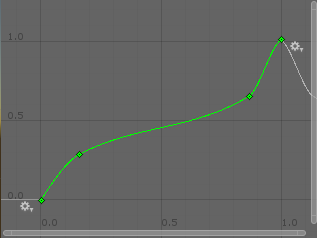
\includegraphics[width=.75\textwidth]{images/BoomerangAnimationCurve}
  \caption[Boomerang animation curve using Unity's built in type]{This curve shows the change in \textbf{\textit{t}} as time goes from 0 to 1 on the x axis using Unity's \emph{AnimationCurve} type.}
  \label{fig:boomerangcurve0}
\end{figure}

\begin{figure}[tbph]
    \centering
    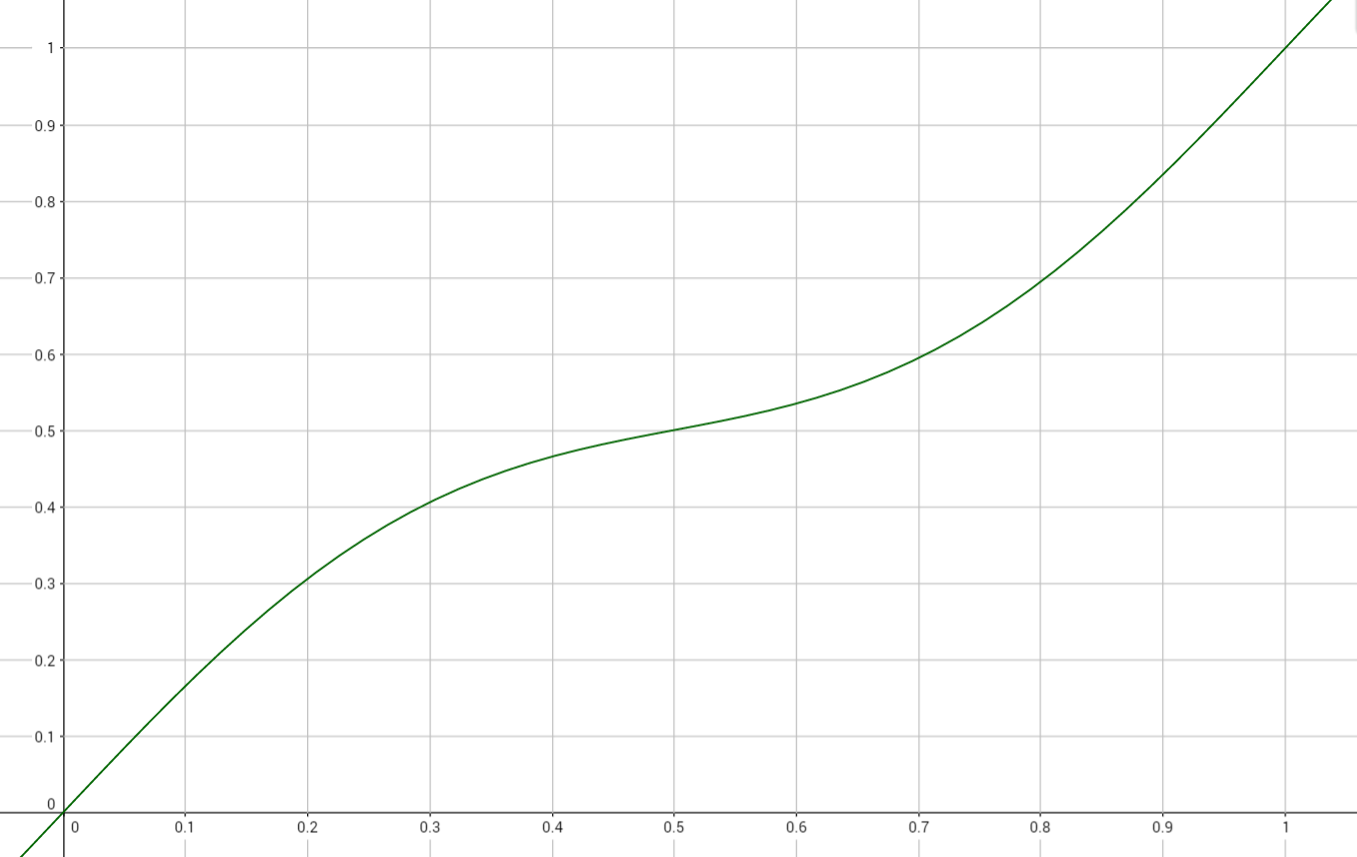
\includegraphics[width=.75\textwidth]{images/BoomerangMathematicalCurve}
    \caption[Boomerang curve using a mathematical formula]{This curve shows the change in \textbf{\textit{t}} as time goes from 0 to 1 on the x axis using the mathematical curve $f(x) = x + sin(6.28x) / 9$}
    \label{fig:boomerangcurve1}
\end{figure}
    
As seen in Figure~\ref{fig:boomerangcurve0}, the \emph{AnimationCurve} approach provides an interface with control points and control point handles which is fairly easy to use, but there is also another way of solving the problem. 

A more generic approach would be to use a mathematical function like $f(x) = x + sin(x) / c$ to create a similar looking curve, but this approach has some problems that need to be dealt with. First of all, the curve needs to be scaled so that the wanted part of it is within the range of [0, 1] for both axes in order for the output to work with the interpolation function. This could be achieved by playing around with a graph plotting tool like \emph{GeoGebra} or similar. In our case, the function $f(x) = x + sin(6.28x) / 9$ as seen in Figure~\ref{fig:boomerangcurve1} would provide similar behaviour to Figure~\ref{fig:boomerangcurve0}, but still lack the strong acceleration towards the end of the interpolation. This approach gives less control to the developers who work in the engine and spending time trying to scale the curves can be quite time consuming.

We also made sure to check the performance difference between the two approaches by measuring the execution time of both. We measured the time spent on each function per update and calculated the mean of the time values after 10 boomerang throws. This gave us the following results:

\begin{itemize}
    \item The average execution time of the \emph{AnimationCurve}'s evaluation function took \textasciitilde$ 0.36 \mu s$
    \item The average execution time of the math function took \textasciitilde$ 0.20 \mu s$.
\end{itemize}

The time difference was calculated using Unity's \emph{Time.realTimeSinceStartup} variable. The \emph{Time.realTimeSinceStartup} float is measured in seconds so we multiplied the average time difference by $10^6$ and used a output precision of two decimals for these results. 
The mathematical approach provides a small increase in performance as seen from the results, but in our case the difference is too small to warrant using it. The \emph{AnimationCurve} approach is far easier to work with directly in the editor instead of using external graph tools to modify the curve to our needs. On the contrary, the mathematical approach is more generic and might see use in non Unity applications.

\section{Interpolation using coroutines}
Interpolations in Unity are generally handled in each script's \emph{Update()} function through the use of timer variables and adding Time.deltaTime to these per update. In some cases this adds unnecessary logic to the update loop of a component and the developer might wish to further decouple the interpolation from the loop itself to improve code readability. This can be handled using C\# coroutines as these functions are capable of stopping execution during a frame and then resuming the next frame to provide similar functionality to that of the standard Unity update loop callback. 

An example of how this is implemented can be seen in the \emph{FieldOfView} component that contains a coroutine for interpolating the view radius of the component:
\begin{minted}[fontsize=\footnotesize]{csharp}
public float viewRadius;

private IEnumerator ViewRadiusLerp(float targetRadius, float speed) {
    while (Mathf.Abs(targetRadius - viewRadius) > 0.1f) {
        viewRadius = Mathf.Lerp(viewRadius, targetRadius, speed * Time.deltaTime);
        yield return null;
    }

    viewRadius = targetRadius;
}
\end{minted}
This function will stop at the end of each while loop execution and resume on the next frame using \emph{yield return null;}. This allows the interpolation to move forwards each frame although the example function in particular will not provide fully linear interpolation. This is due to fluctuations in deltaTime between frames and the observed behaviour of an interpolation using this function will appear as a smooth interpolation that slows down towards its end. A different way of implementing the interpolation, this time in an actually linear fashion would be to use a local timer variable that moves in the range of [0, 1] by adding Time.deltaTime each frame. A modified version of the radius interpolation using this thought process would look like this:
\begin{minted}[fontsize=\footnotesize]{csharp}
public float viewRadius;

private IEnumerator ViewRadiusLerp(float targetRadius, float speed) {
    float lerpTimer = 0;
    while (lerpTimer <= 1f) {
        lerpTimer += Time.deltaTime * speed;
        viewRadius = Mathf.Lerp(viewRadius, targetRadius, lerpTimer);
        yield return null;
    }

    viewRadius = targetRadius;
}
\end{minted}

A benefit of decoupling interpolations from the update loop is that there is no need for an additional conditional variable that checks whether an interpolation is active per frame. When reading the code, the interpolation approach also makes it more clear when the interpolation starts using the \emph{StartCoroutine()} function. 
An apparent thought when working with coroutines and interpolation is the possibility of providing a generic solution for all basic interpolations by using of a static utility class. This will not work as Unity requires that all coroutines need to exist in classes deriving from \emph{MonoBehaviour} which is incapable of being static. This can be worked around by having a singleton \emph{MonoBehaviour} class and call functions through its static instance. 

\section{Initial game balancing}
The full game functionality required for proper user testing ended up being implemented rather late into the project's development. Due to this we had limited time for user testing and needed to provide the testers with a build that already had some initial balancing done. 
\emph{Dockit League} is an asymmetrical game due to the variety of available docking kits so we used a mathematical model~\cite{schell2014art} for the initial balance iteration. Doing so allowed us to have a overview over the different kits including their strengths and weaknesses.

\begin{table}[tbph]
\centering
\caption{Initial balance table}
\label{tab:initBalance}
\begin{tabular}{@{}llllll@{}}
\toprule
\textbf{Docking Kit} & \textbf{Health} & \textbf{Movement Speed} & \textbf{Damage} & \textbf{Utility} & \textbf{Totals} \\ \midrule
Boomerang Kit        & Low (1)         & High (3)                & High (3)        & Medium (2)       & 9               \\
Brawler Kit          & High (3)        & Low (1)                 & Medium (2)      & Medium (2)       & 8               \\
Bomber Kit           & Medium (2)      & Low (1)                 & High (3)        & Medium (2)       & 8               \\
Marksman Kit         & Medium (2)      & Medium (2)              & Medium (2)      & Medium (2)       & 8               \\
Sniper Kit           & Medium (2)      & Medium (2)              & High (3)        & Medium (2)       & 9               \\
Tank Kit             & High (3)        & Low (1)                 & Low (1)         & High (3)         & 8               \\
Trapper Kit          & Low  (1)        & Medium (1)              & Medium (2)      & High (3)         & 8               \\
Support Kit          & Medium (2)      & Medium (2)              & Low (1)         & High (3)         & 8               \\ \bottomrule
\end{tabular}
\end{table}

Balance Table~\ref{tab:initBalance} contains columns for kit name, kit health, kit movement speed, damage and utility. The damage column has values assigned based on the potential damage output of the kit while the utility column has values assigned based on the overall the utility the kit provides through its abilities. This includes abilities that apply modifiers and other effects without necessarily focusing on damage. Further tweaking on cooldowns, damage values and modifier durations is the focus of the user testing rather than the initial balancing as this Section is supposed to give a rough estimate of each kit's capabilities. 
Additional information on the various docking kits and their abilities can be found in Section~\ref{sec:dockingKits}

\subsection{Observations from the initial balance table}     
As seen in Table~\ref{tab:initBalance}, the sniper and boomerang kits end up with a slightly higher total than the other kits. This is a deliberate decision as both kits have a high damage potential if played well while having a low to medium damage potential otherwise. We believe that both kits are fairly challenging to play in order to achieve their full damage potential so the difficulty offsets the the fact that the two kits are a bit stronger than the rest. 
The boomerang kit requires the player to hit with multiple boomerangs while they move forwards and then again once they move back for the maximum amount of damage. The sniper kit requires time and preparation before shooting and rewards a large amount of damage if the projectile actually connects.  
These parts of the two kits allows us to provide a high risk, high reward ratio for playing well.

An interesting thing to note with our current design is that none of the implemented kits have a low utility value. All the kits feature at least 2 abilities that provide utility through either the use of modifiers or other effects. The utility abilities for the kits are generally designed to help patch up the weaknesses of each kit. The brawler kit for example struggles fighting ranged enemies due to its low speed and melee weapon, but contains abilities for reflecting projectiles and stunning opponents to get closer. If any future development were to take place on the project, creating kits with less utility and a larger focus on the other statistics could improve the variety of of the kits.

One important aspect of game balance is the fact that distinct weaknesses is a great way to provide counterplay and avoiding dominant strategies~\cite{gameBalanceWeaknesses}. While the kits generally have abilities that help them somewhat with their weaknesses, these abilities have long enough cooldowns to not always be available. Balancing cooldowns isn't the only way to expose the weaknesses of kits though. 
The boomerang kit is the only kit with low health and has a large damage potential with high movement speed. One of the weaknesses of the boomerang kit is the low health and being caught unaware by enemy players will lead to a swift death. The limited field of view also helps creating situations where the player might have been inattentive and not seen an enemy sneaking in from behind. The high speed of the kit might be seen as beneficial, but can result in the player carelessly rushing into enemies who are right around the corner of walls and other obstacles. 

Another thing to note about the balance table is that it does not take shop price into account. This is due to the fact that we were unsure of how strong each kit was before performing playtesting so we kept the same price for all docking kits. Starting to think of price as part of the initial balance table would allow for certain kits to be stronger than others by justifying their strength with a higher price. Given a larger pool of docking kits fulfilling similar roles than currently implemented in the game, the price could end up being used to a larger extent to create more variety for kits with similar use cases. 
 
\section{Controller based menu navigation in Unity}
\emph{Dockit League} originally had a different main menu and lobby handling script that was more integrated for controllers, but we ended up having to cut it from the last iteration of the game as there was limited time to integrate it with the new lobby and main menu that supported different game modes. We would like to spend some time detailing the old implementation in this section as it might provide additional insight into how controller based menu navigation can be handled in Unity. 

There are two primary things that should be handled differently to accommodate for controller navigation compared to just navigating with the mouse:
\begin{enumerate}
    \item The controller needs an entry point for navigation compared to the mouse. These usually consist of clickable buttons and can be navigated through using the dpad or left analog stick of the controller. 
    \item While having a back button on menu screens is common for mouse and touch navigation, controller users might find it more intuitive to be able and navigate backwards using a physical button. One needs only look back at the era of the \emph{Super Nintendo Entertainment System} and its games to see that developers already were using a physical button for backwards menu navigation. 
\end{enumerate}

Backwards menu navigation can be handled in multiple ways. The current implementation in \emph{Dockit League} allows for arbitrary menu navigation and works well with mice while the old implementation used a stack instead, inspired by how \emph{Android} handles backwards navigation using its fragment back stack~\cite{androidBackStack}. 

The stack based approach allows for simple controls when using the \emph{OnClick} interface to handle individual button presses. The developer simply has to drag the next menu object as a parameter to the menu handling script and the script then takes care of putting the old menu panel into the stack. Once the new menu panel had been displayed the script would quickly look for buttons and set the first found button as the selected one, providing an automated entry point for controller navigation. 

This old implementation also supported adding properties to the top of the stack, allowing custom behaviour on backwards navigation. We handled this by storing enums with the menu stack objects and perform custom behaviour depending on the enum of the popped menu. This was particularly useful for telling Unity to stop hosting or matchmaking whenever the player left certain types of menus. 
The stack based approach also made it easy to use physical buttons for backwards navigation as all the script needed to do was to wait for the correct button to be pressed and then trigger a backwards navigation by popping the stack. 